\begin{filecontents*}[overwrite]{spconf.sty}

\renewcommand{\sfdefault}{phv}
\renewcommand{\rmdefault}{ptm}
\renewcommand{\ttdefault}{pcr}

\oddsidemargin  -6.2truemm
\evensidemargin -6.2truemm

\topmargin 0truept
\headheight 0truept
\headsep 0truept
\textheight 229truemm
\textwidth 178truemm

\twocolumn
\columnsep 6truemm
\pagestyle{empty}

\emergencystretch=11pt

\def\ninept{\def\baselinestretch{.95}\let\normalsize\small\normalsize}

\def\maketitle{\par
 \begingroup
 \def\thefootnote{}
 \def\@makefnmark{\hbox
 {$^{\@thefnmark}$\hss}}
 \if@twocolumn
 \twocolumn[\@maketitle]
 \else \newpage
 \global\@topnum\z@ \@maketitle \fi\@thanks
 \endgroup
 \setcounter{footnote}{0}
 \let\maketitle\relax
 \let\@maketitle\relax
 \gdef\thefootnote{\arabic{footnote}}\gdef\@@savethanks{}%
 \gdef\@thanks{}\gdef\@author{}\gdef\@title{}\let\thanks\relax}

\def\@maketitle{\newpage
 \null
 \vskip 2em \begin{center}
 {\large \bf \@title \par} \vskip 1.5em {\large \lineskip .5em
\begin{tabular}[t]{c}\@name \\ \@address
 \end{tabular}\par} \end{center}
 \par
 \vskip 1.5em}

\def\title#1{\gdef\@title{\uppercase{#1}}}
\def\name#1{\gdef\@name{{\em #1}\\}}
\def\address#1{\gdef\@address{#1}}
\gdef\@title{\uppercase{title of paper}}
\gdef\@name{{\em Name of author}\\}
\gdef\@address{Address - Line 1 \\
               Address - Line 2 \\
               Address - Line 3}

\let\@@savethanks\thanks
\def\thanks#1{\gdef\thefootnote{}\@@savethanks{#1}}
\def\sthanks#1{\gdef\thefootnote{\fnsymbol{footnote}}\@@savethanks{#1}}

\def\twoauthors#1#2#3#4{\gdef\@address{}
   \gdef\@name{\begin{tabular}{@{}c@{}}
        {\em #1} \\ \\
        #2\relax
   \end{tabular}\hskip 1in\begin{tabular}{@{}c@{}}
        {\em #3} \\ \\
        #4\relax
\end{tabular}}}

\def\@sect#1#2#3#4#5#6[#7]#8{
   \refstepcounter{#1}\edef\@svsec{\csname the#1\endcsname.\hskip 0.6em}
       \begingroup \ifnum #2=1\bf\centering
          {\interlinepenalty \@M
             \@svsec\uppercase{#8}\par}\else\ifnum #2=2\bf
          \noindent{\interlinepenalty \@M \@svsec #8\par}\else\it
          \noindent{\interlinepenalty \@M
             \@svsec #8\par}\fi\fi\endgroup
       \csname #1mark\endcsname{#7}\addcontentsline
         {toc}{#1}{\protect\numberline{\csname the#1\endcsname} #7}
     \@tempskipa #5\relax
     \@xsect{\@tempskipa}}

\def\abstract{\begin{center}
{\bf ABSTRACT\vspace{-.5em}\vspace{0pt}}
\end{center}}
\def\endabstract{\par}

\def\keywords{\vspace{.5em}
{\bfseries\textit{Index Terms}---\,\relax%
}}
\def\endkeywords{\par}

\def\copyrightnotice#1{\gdef\@copyrightnotice{#1}}
\let\@copyrightnotice\relax
\def\toappear#1{\gdef\@toappear{#1}}\let\@toappear\relax

\newif\if@preprint\@preprintfalse
\@namedef{ds@preprint}{\global\@preprinttrue}
\@options
\def\ps@preprint{\def\mypage{}\let\@mkboth\@gobbletwo\def\@oddhead{}
  \def\@oddfoot{\rlap{\@toappear}\hfil\mypage\hfil
    \llap{\@copyrightnotice}
    \gdef\mypage{\thepage}\gdef\@toappear{}\gdef\@copyrightnotice{}}}

\if@preprint\ps@preprint
\else\ps@empty\flushbottom\fi

\def\thebibliography#1{\section{References}\list
 {[\arabic{enumi}]}{\settowidth\labelwidth{[#1]}\leftmargin\labelwidth
 \advance\leftmargin\labelsep
 \usecounter{enumi}}
 \def\newblock{\hskip .11em plus .33em minus .07em}
 \sloppy\clubpenalty4000\widowpenalty4000
 \sfcode`\.=1000\relax}
\let\endthebibliography=\endlist

\long\def\@makecaption#1#2{
 \vskip 10pt
 \setbox\@tempboxa\hbox{#1. #2}
 \ifdim \wd\@tempboxa >\hsize #1. #2\par \else \hbox
to\hsize{\hfil\box\@tempboxa\hfil}
 \fi}

\def\fnum@figure{{\bf Fig.\ \thefigure}}
\def\fnum@table{{\bf Table \thetable}}

\flushbottom

\end{filecontents*}

\documentclass{article}
\usepackage[T1]{fontenc}
\usepackage{spconf,amsmath,amsthm,graphicx,booktabs,url,cite}

\graphicspath{{./}{figures/}}  %

\setlength{\textfloatsep}{6pt plus 2pt minus 2pt}
\setlength{\floatsep}{8pt plus 2pt minus 2pt}
\setlength{\intextsep}{8pt plus 2pt minus 2pt}

\makeatletter
\gdef\@title{\fontsize{14}{16}\selectfont
  \uppercase{Inapplicable Components in Audio Anti-Spoofing:
             Metric Identifiability Under Component Pooling}}
\makeatother

\name{\begin{tabular}{@{}c@{}}
  Md.~Shakhoyat Rahman Shujon\textsuperscript{1} \quad
  Khadimul Islam Mahi\textsuperscript{1} \quad
  Md.~Milon Islam\textsuperscript{1} \\
  Md~Rezwanul Haque\textsuperscript{2} \quad
  Fakhri Karray\textsuperscript{2,3}
\end{tabular}}
\address{%
  \textsuperscript{1}Department of Computer Science and Engineering,
        Khulna University of Engineering \& Technology \\
  \textsuperscript{2}Department of Electrical and Computer Engineering, University of Waterloo \\
  \textsuperscript{3}Department of Machine Learning,
        Mohamed bin Zayed University of Artificial Intelligence \\
  {\small\normalfont
   skt104.shujon@gmail.com \quad mahi.jess9t9@gmail.com \quad
   milonislam@cse.kuet.ac.bd \quad rezwan@uwaterloo.ca \quad karray@uwaterloo.ca}}

\begin{document}
\maketitle

\begin{abstract}
Component-level anti-spoofing scores a recording's speech and environment on separate axes. An
untouched capture has no separable component, so both attributes are inapplicable; the ESDD2
protocol counts such clips as bona fide on both axes. We show that this stated rule breaks the equal
error rate (EER) it reports. For one fixed model, changing only inapplicable clips' score moves the
environmental EER from $0.5382$ to $0.1412$. We prove that pooling these clips mixes ROC curves:
weighted-area summaries such as AUC survive; EER admits no aggregation rule. A published pooled EER
leaves the component-only EER in an interval, and these intervals separate no pair of eleven
challenge systems. Neither per-clip reduction nor training on the stated rule repairs this; such
training lowers the reported EER by $0.20$ without improving component detection. The organiser
holds the partition, so the fix is a one-line scorer change.
\end{abstract}

\begin{keywords}
audio anti-spoofing, speech deepfake detection, component-level detection,
evaluation protocols, equal error rate
\end{keywords}

\section{Introduction}
\label{sec:intro}

Audio deepfake detection increasingly asks not whether a recording is manipulated but which part
of it is. Partial-spoof detection localises manipulation in time~\cite{partialspoof}.
Component-level detection localises it by source, scoring a speech component and an environmental
component on separate axes~\cite{compspoof2026,esdd2,pcmix2026}. Separating the axes is useful
because a convincing forgery may generate only one of them. A system that reports which component
was synthesised says more than one that reports a single verdict.

\textbf{Two kinds of zero.} A bona fide mixture contains a separate speech object. Its source is
defined, and it happens to be genuine. An untouched capture contains no separate object, so the
question of its source has nothing to refer to. Zero-inflated models draw exactly this line. A
\emph{structural} zero is a subject not at risk. A \emph{random} zero is one that could have
responded and did not. Treating them alike biases the result~\cite{he2014zeros}.

\textbf{The ESDD2 protocol decides this explicitly.} It treats the two zeros alike. Its Table~I maps
class $0$ (\texttt{original}) to \emph{bona fide} on both the speech and the environmental
axis~\cite{esdd2plan}, and the released scorer implements that mapping. We are therefore not
exposing an unstated rule. We show that the rule pools the inapplicable clips with the applicable
ones against a shared negative set. The pooling then destroys the metric it reports. Holding a model
fixed and varying only the constant assigned to those clips moves its reported environmental EER
from $0.5382$ to $0.1412$ (\S\ref{sec:exp}). The spread is $0.40$, under a rule every team follows
identically.

\textbf{Which metrics survive this?} The inapplicable clips join the positive side while the
negative set is unchanged. Pooling therefore adds ROC curves pointwise (Fig.~\ref{fig:pooling}), so
areas average. We show the converse: exactly the weighted-area family aggregates
(\S\ref{sec:unrec}). A threshold crossing such as the equal error rate does not.

\vspace{2pt}\noindent \textbf{Contributions.} (i) We prove the converse of a known area
identity~\cite{gonen2013}: under this pooling, only monotone transforms of a weighted area admit an
aggregation rule. AUC admits one. EER admits none of any form. (ii) We bound the component-only EER
given a published pooled EER. It separates two systems only when their published EERs differ by more
than the inapplicable share, and on ESDD2 it separates no pair among eleven systems. (iii) We derive
what the released scorer reports when all inapplicable clips share one score. No participant-side
remedy works: no per-clip reduction computes the component-only EER, and training on the stated rule
lowers the reported value by $0.20$ with no gain in component detection. (iv) We show that the
repair belongs at the scorer, which already holds the partition. An outside reader can still audit a
published EER from the submitted scores alone, cutting its error from $0.2246$ to $0.0068$ on the
reference system.

The setting is the ESDD2 challenge~\cite{esdd2} and its CompSpoofV2
corpus~\cite{compspoof2026}. Four of five classes are mixtures whose components each carry a
provenance label. The fifth, class $0$ (\texttt{original}), is an untouched capture, $52.8\%$ of the
environmental bona fide side on the test split. We call it \emph{inapplicable} throughout, and
reserve \texttt{original} for the score column of that name in the submission format.

\section{Metric identifiability under component pooling}
\label{sec:unrec}

Fix a component axis with negative set $\mathcal{N}$ and positive side $\mathcal{P} =
\mathcal{P}_0 \sqcup \mathcal{P}_{\mathrm{a}}$, where $\mathcal{P}_0$ collects the inputs the axis
does not describe. Write $w_0 = |\mathcal{P}_0|/|\mathcal{P}|$ and $w_{\mathrm{a}} = 1-w_0$. The
published protocol scores $\mathcal{P}$ against $\mathcal{N}$, a reader removing the mapping
scores $\mathcal{P}_{\mathrm{a}}$ against \emph{the same} $\mathcal{N}$. Only the positive side
changes, so with $\mathrm{FRR}_S$ the false-rejection rate on $S$,
\begin{equation}
\mathrm{FRR}_{\text{pub}}(\tau) \;=\; w_0\,\mathrm{FRR}_0(\tau) \;+\; w_{\mathrm{a}}\,\mathrm{FRR}_{\mathrm{a}}(\tau).
\label{eq:mix}
\end{equation}

Because $\mathcal{N}$ is shared, the threshold at a given false-acceptance rate $t$ is a functional
of $\mathcal{N}$ alone, so the same weights carry to the curves,
\begin{equation}
\mathrm{ROC}_{\mathrm{pub}}(t) \;=\; w_0\,\mathrm{ROC}_0(t) \;+\; w_{\mathrm{a}}\,\mathrm{ROC}_{\mathrm{a}}(t),
\label{eq:roc}
\end{equation}
and pooling an inapplicable class is convex combination in ROC space. The question is which
summaries commute with it.

\begin{figure}[!t]
\centering
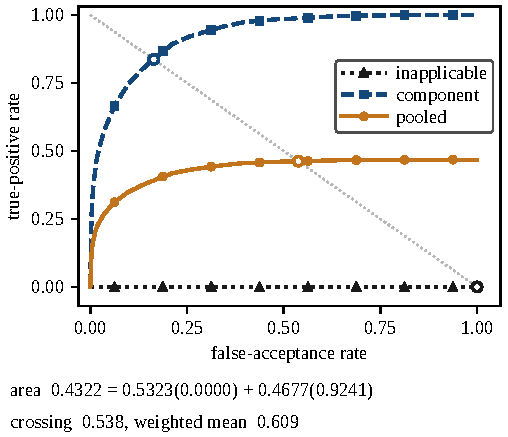
\includegraphics[width=\columnwidth]{fig_pooling}
\caption{\textbf{Areas average; crossings do not.} Pooling an inapplicable class adds ROC curves
pointwise, which is \eqref{eq:roc}, so the pooled area is exactly the weighted mean of the component
areas while the pooled crossing is not the weighted mean of theirs. BEATs probe at seed $1337$,
environmental axis, evaluation split, inapplicable rows held at $c=0$. $R_0$ is a step because every inapplicable clip
carries one score, and \eqref{eq:roc} assumes no continuity, so this is an instance of it and not of the
curve class Theorem~1 quantifies over.}
\label{fig:pooling}
\end{figure}

\vspace{2pt}\noindent\emph{Intuition.} Pooling adds ROC curves pointwise, so areas average.
Threshold crossings need not: the crossing of a sum is not the sum of the crossings.

\vspace{2pt}\noindent\textbf{Theorem 1 (collapsibility).} \emph{Let $T$ be a ROC summary,
continuous and strictly monotone under pointwise dominance on a convex class $\mathcal{R}$
whose image $T[\mathcal{R}]$ is an interval and on which every quadruple in $T[\mathcal{R}]^4$
is realised by four curves. Then $T$ admits an aggregation rule $T_{\mathrm{pub}} = \varphi(T_0,
T_{\mathrm{a}}, w_0)$ for all curves and all $w_0$ if and only if $T = g \circ L$ with $g$
continuous and strictly monotone and $L[\mathrm{ROC}] = c + \int_0^1 \mathrm{ROC}\,dW$ for a fixed
signed measure $W$, in which case $\varphi$ is the quasi-arithmetic mean generated by $g^{-1}$.}

\begin{proof}
\emph{Sufficiency.} With $T=g\circ L$ and $w_0+w_{\mathrm{a}}=1$ the constant is absorbed, so $L$ is
affine under mixing; writing $L=g^{-1}\!\circ T$ and applying $g$ gives the rule with
$\varphi(x,y,w)=g\big(w\,g^{-1}(x)+(1-w)g^{-1}(y)\big)$.

\emph{Necessity.} Fix $w$ and set $x\oplus y=\varphi(x,y,w)$ on $I=T[\mathcal{R}]$. Mixing is
idempotent, so $x\oplus x=x$; $\oplus$ is strictly increasing in each argument because mixing
preserves pointwise dominance; and it is bisymmetric, since $(A\oplus B)\oplus(C\oplus D)$ and
$(A\oplus C)\oplus(B\oplus D)$ are both $w^2A+w(1-w)(B+C)+(1-w)^2D$. Continuity is inherited from
$T$, and the richness hypothesis carries all four to $I^4$. Acz\'el~\cite{aczel1966} then gives a
continuous strictly monotone $k_w$ and $\alpha(w)\in(0,1)$ with $x\oplus y=k_w^{-1}\big(\alpha(w)
k_w(x)+(1-\alpha(w))k_w(y)\big)$. Mixing at $v$ after $w$ is mixing at weights $vw,\,v(1-w),\,1-v$,
so $\{\oplus_w\}$ is mutually bisymmetric, which for quasi-arithmetic means forces a common
generator $k$; idempotence and the same composition then make $\alpha$ multiplicative and
continuous, so $\alpha(w)=w$. Hence $k\circ T$ is affine and continuous on $\mathcal{R}$, giving the
integral representation with $g:=k^{-1}$.
\end{proof}

\noindent The dividing line the theorem predicts is checked numerically in the released code.

\vspace{2pt}
\noindent\emph{Relation to prior work.} The integral class is not new~\cite{wieand1989}, and
characterisations of the same shape exist for confusion counts~\cite{prati2026}, association
measures~\cite{kenah2025}, and fairness auditing under unobserved protected
class~\cite{kallus2019}. Those aggregate over groups carrying their own negatives. A positive
population mixed against a common reference is known to give a mixture of ROC curves, which
is~\eqref{eq:roc}~\cite{gonen2013}. What is new is the converse: which summaries admit any
aggregation rule, and that a threshold crossing admits none.

\vspace{2pt}
The theorem sorts the summaries in routine use. Area under the curve, partial area, and
true-positive rate at a fixed false-acceptance rate are of this form, as is a detection cost at a
\emph{fixed} threshold. The equal error rate is not, nor is a minimum detection cost (a minimum of
functions affine in the share, hence concave in it) nor Youden's index (a maximum, hence convex).
We measure this on both axes over seven systems: the reference baseline, frozen BEATs, SSLAM,
XLS-R and EAT probes, a BEATs attentive head and the two-encoder. All but SSLAM and XLS-R are rows
of Table~\ref{tab:spread}. Every summary the theorem calls collapsible has a residual at machine
precision, and every one it does not has a residual of at least $1.4\times10^{-4}$. Taking $W$
Lebesgue recovers the area~\cite{hanley1982}. The residual is an exact algebraic difference, not a
statistical test. An equal error rate is a fixed point of $\mathrm{FAR}=\mathrm{FRR}$ rather than an
integral against the curve, and the fixed point of a convex combination is not the combination of
the fixed points.

\vspace{2pt}\noindent\textbf{Theorem 2 (sharp partial identification).} \emph{A published table
fixing $w_0$ and $\mathrm{EER}_{\text{pub}}$ confines the component-only value to}
\begin{equation}
\Big[\max\Big(0,\tfrac{\mathrm{EER}_{\text{pub}} - w_0}{w_{\mathrm{a}}}\Big),\;
      \min\Big(1,\tfrac{\mathrm{EER}_{\text{pub}}}{w_{\mathrm{a}}}\Big)\Big],
\label{eq:interval}
\end{equation}
\emph{and both endpoints are attained, so the interval is the sharp identified set.}

\noindent Write $t^\ast$ for the threshold at which the published rates cross, so
$\mathrm{FAR}(t^\ast) = \mathrm{FRR}_{\text{pub}}(t^\ast) = \mathrm{EER}_{\text{pub}}$. Evaluating
\eqref{eq:mix} there, with $\mathrm{FRR}_0(t^\ast) \in [0,1]$ the only freedom, gives
$\mathrm{FRR}_{\mathrm{a}}(t^\ast) \in [(\mathrm{EER}_{\text{pub}} - w_0)/w_{\mathrm{a}},\,
\mathrm{EER}_{\text{pub}}/w_{\mathrm{a}}]$. Because $\mathcal{N}$ is shared the false-acceptance
rate is common to both components, so $\mathrm{FAR}_{\mathrm{a}}(t^\ast) =
\mathrm{EER}_{\text{pub}}$; since $\mathrm{FAR}$ falls and $\mathrm{FRR}_{\mathrm{a}}$ rises in
$t$, the component-only crossing $\mathrm{EER}_{\mathrm{a}}$ lies between
$\mathrm{FAR}_{\mathrm{a}}(t^\ast)$ and $\mathrm{FRR}_{\mathrm{a}}(t^\ast)$. As
$(\mathrm{EER}_{\text{pub}} - w_0)/w_{\mathrm{a}} \le \mathrm{EER}_{\text{pub}} \le
\mathrm{EER}_{\text{pub}}/w_{\mathrm{a}}$ whenever $\mathrm{EER}_{\text{pub}} \le 1$, that bracket
is contained in \eqref{eq:interval}; intersecting with $[0,1]$ gives the stated form. Both
directions are checked numerically in the released code.

\noindent\emph{Interpretation.} Given only the pooled EER and the inapplicable share, the
component-only value is an interval, not a point.

Both endpoints are attained, so \eqref{eq:interval} is the sharp identified set given
$(w_0,\mathrm{EER}_{\text{pub}})$: for every sampled value in it, endpoints included, the released
code builds an admissible system matching both crossings to $10^{-12}$. Fixing the \emph{other}
published cells of a particular submission constrains the construction further, and there a witness
exists for the lower endpoint but none is claimed for the upper. Bounding a component functional
under a two-component mixture is classical~\cite{horowitz1995}. \eqref{eq:interval} bounds from a
single published scalar. The reference baseline's environmental row on the \emph{evaluation} split
has $w_0=0.5323$ and $\mathrm{EER}_{\text{pub}}=0.4336$, so \eqref{eq:interval} returns
$[0,\,0.9271]$. That is $93\%$ of the range, and it contains the true $0.2090$ along with almost
everything else.

On the \emph{test} split, across the eleven systems publishing component EERs in the challenge
overview, \eqref{eq:interval} determines \emph{none} of the $\binom{11}{2}=55$ pairwise comparisons
on either axis. Every interval has lower endpoint $0$, so all eleven share a common sub-interval and
every strict ordering of the eleven remains feasible. Two intervals from \eqref{eq:interval} are
disjoint only when the published EERs differ by more than $w_0$. The largest published gaps are
$0.3410$ on the environmental axis and $0.2402$ on speech, against $w_0 = 0.5282$ and $0.3961$.
After publication, the component-only EER cannot be recovered.

\section{Limits of per-clip score reduction}
\label{sec:method}

Section~\ref{sec:unrec} shows a published table does not determine the component-only value. A
natural reading is that the fault is one of disclosure. Teams should state which fill value they
used, and a reader holding the per-clip scores could then undo it. That reading is wrong. The
information is not missing. A scorer holding the per-clip scores and the corpus labels can compute
the component-only value directly, and \S\ref{sec:exp} reports it. What fails is the \emph{format}.
A submission carrying one number per axis forces a reduction before scoring, and no reduction rule
computes the component-only value.

\subsection{Applicability signal in the submission format}

The submission format carries a predicted class and three scores, one of them the
score for \texttt{original}~\cite{esdd2plan}. That score is not an applicability
declaration, because the format has no such field. But a per-clip applicability signal can be read
off it, and a strong one: on the reference system it separates the inapplicable class at an AUC of
$0.9964$. The information is present in every
submitted file, and the scorer uses none of it. Writing $\gamma_a$ for
a system's posterior that axis $a$ applies and $d_a$ for its authenticity score, a
format accepting one number per axis forces a reduction $\tilde{s}_a = \gamma_a d_a
+ (1-\gamma_a)c$.

On the reference system's environmental axis the published value is $0.4336$ and the
component-only value is $0.2090$. No fill value reaches $0.2090$. The constant $c=0$ gives $0.4654$,
and $c=0.5$ gives $0.1307$, the Proposition~3 floor. An \emph{oracle} gate handed the exact
partition gives the same, because a perfect gate reduces to that constant. A gate built from the
submitted \texttt{original} score gives $0.1355$. Sweeping every constant does not help: as $c$
rises past $0.0119$ the reported value drops from $0.4631$ to $0.1970$, the closest any constant
comes. The quantity is not a function of what the format carries, so this is an identification
problem, not an estimation one.

\begin{table}[!tb]
\centering
\caption{\textbf{Environmental EER under three declared constants for the inapplicable rows},
model held fixed, evaluation split. Only $c$ changes within a row; the systems' own score scales
differ, and $c$ is not rescaled to match them. \texttt{prior} is the third declared constant, the share of the
applicable clips that are bona fide on this axis. Cells are means over three seeds, with seed standard deviation at most $0.0015$
except on the attentive head, whose seeds straddle a step (\S\ref{sec:fill}). The reference row is
one released checkpoint scored on its native scale. Its $c=0$ cell sits near a step too: in $6\%$ of
$1{,}000$ class-stratified resamples it falls to about $0.20$, and its spread falls with it. Spreads are computed before rounding, so the
reference row reads $0.3346$ where its displayed cells differ by $0.3347$; the other four rows agree
either way. That system's own published value, with its own scores on the inapplicable rows rather
than a constant, is $0.4336$ (Table~\ref{tab:endtoend}), which no cell here reproduces.
The component-only column is the value with the inapplicable class removed; it is identical at all three constants, so its own spread is exactly
$0$.}
\label{tab:spread}
\setlength{\tabcolsep}{2.0pt}\small
\begin{tabular}{@{}lcccrc@{}}
\toprule
 & \multicolumn{3}{c}{Env-EER at $c=$} & & component \\
\cmidrule(lr){2-4}
system & $0$ & $0.5$ & prior & spread & only \\
\midrule
BEATs probe    & $0.5382$ & $0.1412$ & $0.1517$ & $\mathbf{0.3970}$ & $0.1632$ \\
EAT probe      & $0.5400$ & $0.1600$ & $0.1677$ & $0.3800$ & $0.1900$ \\
attentive head & $0.4529$ & $0.3515$ & $0.3561$ & $0.1014$ & $0.1569$ \\
two-encoder    & $0.1041$ & $0.1010$ & $0.1016$ & $0.0031$ & $0.1559$ \\
reference      & $0.4654$ & $0.1307$ & $0.1307$ & $0.3346$ & $0.2090$ \\
\bottomrule
\end{tabular}
\end{table}

\subsection{Why no reduction can work}

\vspace{1pt}\noindent\textbf{Proposition 3.} \emph{No reduction rule computes the component-only equal
error rate. The infimum over assignments solves $\mathrm{FAR} =
w_{\mathrm{a}}\mathrm{FRR}_{\mathrm{a}}$, whereas the component-only value solves $\mathrm{FAR} =
\mathrm{FRR}_{\mathrm{a}}$; the two fixed points differ whenever $w_{\mathrm{a}}<1$.}

\noindent A reduction changes ranks but cannot remove rows from $\mathcal{P}$, which the protocol
fixes. By \eqref{eq:mix} the infimum over assignments is attained at $\mathrm{FRR}_0 = 0$, where
the equal error condition reads $\mathrm{FAR} = w_{\mathrm{a}}\mathrm{FRR}_{\mathrm{a}}$; since
$w_{\mathrm{a}} < 1$ and the two rates are oppositely monotone, that fixed point lies strictly
below the one solving $\mathrm{FAR} = \mathrm{FRR}_{\mathrm{a}}$.

\vspace{2pt}
The gap is not asymptotic. On the reference system's environmental axis,
$w_{\mathrm{a}} = 0.4677$. Ranking every inapplicable row above every threshold gives $0.1307$. The
fixed point of $\mathrm{FAR} = w_{\mathrm{a}}\mathrm{FRR}_{\mathrm{a}}$ is $0.1307$ to four
decimals, against a component-only value of $0.2090$. A system that reduces optimally does not
approach the right answer. It converges on a different one. A particular assignment may
\emph{coincide} numerically: the released code shows one matching to $5\times10^{-6}$. But an
assignment built from the answer computes nothing, so the proposition concerns rules, not
numbers.

Zhou and Wang~\cite{zhou2026eer} show a neighbouring invariance under monotone score transforms
with the support held fixed. Proposition~3 is the complement.

\vspace{2pt}\noindent\emph{Why not simply report AUC?} It is collapsible, so it would work. But EER
is the operating-point summary anti-spoofing evaluation is built on, from
ASVspoof~\cite{asvspoof2021,asvspoof5} onward. Replacing it changes the evaluation objective rather
than recovering the component-only EER.

\subsection{Where the burden falls}

Proposition~3 is a statement about participants. A team holding its own per-clip scores cannot
recover the component-only value, whatever constant it declares and however fully it discloses the
choice. The quantity is not a function of what the submission format carries. The obvious response
is to ask teams to report more. That response is unnecessary here, and we do not make it.

The scorer already holds what is needed. The corpus defines the partition, and the released
reference implementation computes it: it is the same indicator the trainer uses to mask the
inapplicable clips out of both component losses. The organisers run the scoring. Nothing has to be
requested from participants, and no field has to be added to the submission format. The component
metric can be computed on the applicable clips directly, which is a one-line change in the
scorer.

The impossibility result is what makes this necessary rather than merely tidy. If a reduction rule
could recover the value, conditional scoring would be one option among several and disclosure would
suffice. Because no rule can, evaluation that reports a component metric over inapplicable inputs
cannot be repaired downstream, and the burden sits with whoever designs the protocol. Sometimes no
partition is available at scoring time, as in cross-corpus evaluation or deployment in the wild.
There the quantity is not identified at all, and the right response is to report a summary the
theorem admits rather than an equal error rate.

This is not selective prediction. There a model declines the inputs it expects to get wrong, and
the trade it manages is coverage against risk~\cite{elyaniv2010}. Here the partition is fixed by
the corpus rather than chosen by the model, and the metric is undefined on those inputs rather than
merely hard.

\section{Experiments}
\label{sec:exp}

\subsection{Setup}

CompSpoofV2~\cite{compspoof2026,esdd2} has $175{,}361$ training and $24{,}864$ validation clips. We
evaluate on the $27{,}605$-clip evaluation set, released with labels after the challenge and
containing generators unseen in training. Clips are provided at several sampling rates, and every
system here resamples to $16$~kHz mono. Systems are frozen encoders with linear or attentive
probes, layers chosen on a generator holdout, at three seeds. Table~\ref{tab:spread} reports five: linear probes on BEATs and on EAT, a
BEATs attentive head, a two-encoder probe reading BEATs for the environmental axis and XLS-R for the
speech axis, and the reference baseline. SSLAM and XLS-R linear probes enter only
\S\ref{sec:unrec}'s collapsibility check. The reference system is the released baseline, the only
external system publishing per-clip scores. \S\ref{sec:unrec}'s eleven-system analysis uses the
published challenge table, which reports scalars only.
Code and per-clip scores reproducing every number: \texttt{github.com/REPLACE}.

\subsection{Fill-value sensitivity}
\label{sec:fill}

Table~\ref{tab:spread} holds each system fixed and varies only the constant assigned to the
inapplicable rows. The reported environmental EER moves by between $0.0031$ and $0.3970$ across the
five systems: two teams submitting the identical model would publish $0.5382$ and $0.1412$. Under the component-only
protocol the same sweep moves every system by exactly zero, because the class is dropped and the
constant has nowhere to act.

All inapplicable clips receive $c$, so $\mathrm{FRR}_{\text{pub}}$ jumps by $w_0$ at $c$, and
\eqref{eq:mix} leaves three regimes. The protocol does not constrain where it can fall. The
submission format asks for confidence scores without specifying a range, and the plan's own worked
example lists $1.22$, $-1.54$ and $-1.89$~\cite{esdd2plan}. Unbounded logits are therefore within
the rules. If $\mathrm{FAR}(c)$ lies above the jump, the atom is rejected and the reported value is at
least $w_0$ (BEATs and EAT at $c=0$). If it lies below, the atom is accepted and the value is the
Proposition~3 floor. In between, the atom captures the operating point. The released scorer averages
$\mathrm{FAR}$ and $\mathrm{FRR}$ at the nearest ROC vertex, so it returns the mean of
$\mathrm{FAR}(c)$ and the nearer end of the jump ($28$ of $39$ cells, to $1.5\times10^{-4}$). That
value steps by $w_0/2 = 0.27$ where $\mathrm{FAR}(c)$ crosses the midpoint of the jump. The
attentive head's seeds straddle that point, so at $c=0.5$ one reports $0.1550$ and another
$0.4706$, while its component-only value stays between $0.1545$ and $0.1611$. The two-encoder's
constants all lie within $0.026$ of the capture/accept boundary, where the average straddles the
floor. Its values sit within $0.0032$ of it. That is a property of where its scores fall, not
evidence that the mapping is harmless.

\subsection{Acoustic difficulty or pooling?}

A reviewer may object that the environmental axis moves further because environmental manipulation
is simply harder to detect. On that reading the pooled value reports a real deficiency rather than a
protocol defect. The ablation separates the two on a fixed model. Scored over the applicable clips
alone, where every clip carries a component annotation, the environment head reaches $0.2090$
against the speech head's $0.1906$. That is a difference of $0.0184$ on the task the axes name.
Admitting the inapplicable clips under the mandated mapping moves the environment axis by $+0.2246$
and the speech axis by $+0.0087$. The model, its scores and the negative set are all unchanged. The heads are comparable at
component detection. Of the $0.2343$ separating the two published values, $0.2159$ ($92\%$) is the
net contribution of pooling, and the remaining $0.0184$ is the difference between the heads. The direction follows the weighted false-rejection gap
$w_0(\mathrm{FRR}_0-\mathrm{FRR}_a)$, evaluated at the published operating threshold $\tau^\ast$.
With $w_0 = 0.5323$ on the environmental axis against $0.3991$ on the speech axis, the gap is
$0.3381$ and $0.0169$. It does not equal the distortion, because the operating threshold also moves
between the two conditions. It does identify which axis the mapping will distort. The reference
trainer masks the inapplicable clips out of both component losses, so neither head was supervised
on them. Their output there is unspecified behaviour, not a measured deficiency.

The free constant exists for any team that masks the inapplicable clips during training, and the
reference trainer is not alone in doing so. The fifth-placed challenge system masks both component
losses on the inapplicable clips as well. Its stated reason is that the component labels are
defined only for applicable audio~\cite{sit2026}. The remaining systems do not document this choice. Systems
trained on the mapping instead are covered by the experiment below.

Training on the mandated mapping does not repair this. We supervise two component heads on inapplicable
clips, changing only the loss mask and holding every other setting fixed. That lowers the reported
environmental value by $0.20$ across three seeds and two frozen-BEATs feature configurations, layer
$7$ alone and layers $7$--$10$ concatenated. Component-only detection does not improve. What the heads acquire is the ability to recognise an
untouched capture, not the ability to detect a synthesised environment. The environmental score's
AUC for the inapplicable class rises from $0.10$ to $0.71$. The reported value settles within
$0.008$ of the $\mathrm{FAR} = w_{\mathrm{a}}\mathrm{FRR}_{\mathrm{a}}$ fixed point of
Proposition~3. The sign of the bias flips. Its existence does not.

\subsection{The applicability signal and a format confound}

Applicability is nearly free here, and the reason is a format artefact. A rule reading the sample
rate alone reaches $\mathrm{F}_1$ $0.9635$, because $93\%$ of inapplicable rows are not $16$~kHz
mono. On the format-matched subset ($525$ rows against $20{,}150$) it collapses to an AUC of exactly
$0.5000$. The reference system's own \texttt{original} score, the signal behind
Table~\ref{tab:endtoend}'s gate, holds at $0.9957$ there. Every mixture is $16$~kHz mono, so this control
constrains applicability, not the component metric. The system identifies the class at an AUC of
$0.9964$ and is nonetheless charged an environmental EER of $0.4336$. The pooling produces that gap.
The gate fits no parameters. But Table~\ref{tab:endtoend} applies it on the full evaluation split,
where these format differences are available to help it, and the control rests on $525$ inapplicable
rows.

\subsection{Applicability-conditioned evaluation}

\begin{table}[!tb]
\centering
\caption{\textbf{What a third party can recover, and what the organiser can.} Reference system,
evaluation split, no retraining. The applicability-conditioned column uses only the signal
already present in the submitted scores, so it is what an outside reader can reconstruct;
component-only is what the organiser computes exactly from the withheld partition. Error is
absolute deviation from that reference, computed before rounding, so the speech row's $0.0019$ is
not the difference of its two displayed cells. Bracketed figures are $95\%$ clustered bootstrap
intervals ($2{,}000$ resamples at a seed fixed in the released code; the cluster is the source
component clip, each untouched capture forming its own): pooled $[0.217, 0.232]$ and
$[0.006, 0.011]$, conditioned $[0.005, 0.009]$ and $[0.000, 0.003]$.
Clustering is close to a no-op on this split, where $80$ of $27{,}605$ rows share an environmental
source; it is reported because it is the correct estimator, not because it changed anything.}
\label{tab:endtoend}
\setlength{\tabcolsep}{3.4pt}\small
\begin{tabular}{@{}lccccc@{}}
\toprule
 & & applic.\ & component & \multicolumn{2}{c}{abs.\ error} \\
\cmidrule(lr){5-6}
axis & pooled & cond. & only & pooled & cond. \\
\midrule
environment & $0.4336$ & $0.2022$ & $0.2090$ & $0.2246$ & $\mathbf{0.0068}$ \\
speech      & $0.1993$ & $0.1886$ & $0.1906$ & $0.0087$ & $\mathbf{0.0019}$ \\
\bottomrule
\end{tabular}
\end{table}

Table~\ref{tab:endtoend} asks how much of the damage is visible from outside. We derive $\gamma_a$
from the submitted \texttt{original} score with no retraining, and score each axis over
$\{x:\gamma_a(x)\ge\tfrac12\}$. The environmental EER is $0.2022$ against a component-only $0.2090$,
and the speech EER $0.1886$ against $0.1906$. The error of a reported value is its absolute
deviation from the component-only value: $0.0068$ and $0.0019$, against $0.2246$ and $0.0087$ under
the pooled protocol. That is a reduction of $97\%$ and $78\%$ in absolute metric error, at precision
$0.999$ and recall $0.943$. Sweeping the threshold from $0.1$ to $0.9$ moves the
environmental error only between $0.0036$ and $0.0096$.

The reading is not that systems should report this signal. It is that the signal is strong enough
for a reader holding a published per-clip submission to \emph{approximately} audit a component EER
that the protocol has made unrecoverable. The organiser, holding the partition, recovers it exactly
and at no cost. That asymmetry is the argument for fixing the metric at the scorer.

\section{Conclusion}
\label{sec:conc}

Component axes create inputs on which an axis is undefined. Pooling them against shared negatives
makes recoverability a property of the summary. Areas aggregate, and the equal error rate does not.
A published EER confines the component value only to an interval. Here a fixed model's environmental
EER moves by $0.3970$, and the interval separates none of the $55$ published comparisons. No
per-clip reduction removes the dependence, because a reported EER is correct only when a system
happens to reject inapplicable clips at exactly its own component error rate. The organiser already
holds the partition. Scoring each component axis on applicable inputs is a one-line scorer change,
and it is the change we recommend.

\begin{thebibliography}{10}

\bibitem{partialspoof}
Lin Zhang, Xin Wang, Erica Cooper, Nicholas Evans, and Junichi Yamagishi,
\newblock ``The {PartialSpoof} database and countermeasures for the detection of short fake speech segments embedded in an utterance,''
\newblock {\em IEEE/ACM Trans. Audio, Speech, Language Processing}, vol. 31, pp. 813--825, 2023.

\bibitem{compspoof2026}
Xueping Zhang, Yechen Wang, Linxi Li, Liwei Jin, and Ming Li,
\newblock ``{CompSpoof}: A dataset and joint learning framework for component-level audio anti-spoofing countermeasures,''
\newblock in {\em Proc. IEEE ICASSP}, 2026, pp. 18067--18071,
\newblock arXiv:2509.15804v2.

\bibitem{esdd2}
Xueping Zhang, Han Yin, Yang Xiao, Lin Zhang, Ting Dang, Rohan~Kumar Das, and Ming Li,
\newblock ``Overview of {ESDD2}: Environment-aware speech and sound deepfake detection challenge,''
\newblock in {\em Proc. IEEE Int. Conf. Multimedia and Expo Workshops (ICMEW)}, 2026,
\newblock arXiv:2606.10791v2, 2026.

\bibitem{pcmix2026}
Zhenshan Zhang, Xueping Zhang, Linxi Li, Yechen Wang, and Ming Li,
\newblock ``{PC-Mix}: Partial-component audio spoofing detection under mixed speech and environmental sound conditions,''
\newblock {\em arXiv preprint arXiv:2607.10345v1}, 2026.

\bibitem{esdd2plan}
Xueping Zhang, Han Yin, Yang Xiao, Lin Zhang, Ting Dang, Rohan~Kumar Das, and Ming Li,
\newblock ``{ESDD2}: Environment-aware speech and sound deepfake detection challenge evaluation plan,''
\newblock {\em arXiv preprint arXiv:2601.07303v5}, 2026.

\bibitem{aczel1966}
J\'{a}nos Acz\'{e}l,
\newblock {\em Lectures on Functional Equations and Their Applications},
\newblock Academic Press, 1966.

\bibitem{gonen2013}
Mithat G\"onen,
\newblock ``Mixtures of receiver operating characteristic curves,''
\newblock {\em Academic Radiology}, vol. 20, no. 7, pp. 831--837, 2013.

\bibitem{wieand1989}
Sam Wieand, Mitchell~H. Gail, Barry~R. James, and Kang~L. James,
\newblock ``A family of nonparametric statistics for comparing diagnostic markers with paired or unpaired data,''
\newblock {\em Biometrika}, vol. 76, no. 3, pp. 585--592, 1989.

\bibitem{prati2026}
Ronaldo~C. Prati,
\newblock ``A unified algebraic framework for classification performance evaluation,''
\newblock {\em arXiv preprint arXiv:2607.04028v2}, 2026.

\bibitem{kenah2025}
Eben Kenah,
\newblock ``Rothman diagrams: the geometry of association measure modification and collapsibility,''
\newblock {\em arXiv preprint arXiv:2506.23927}, 2025.

\bibitem{kallus2019}
Nathan Kallus, Xiaojie Mao, and Angela Zhou,
\newblock ``Assessing algorithmic fairness with unobserved protected class using data combination,''
\newblock {\em Management Science}, vol. 68, no. 3, pp. 1959--1981, 2022.

\bibitem{hanley1982}
James~A. Hanley and Barbara~J. McNeil,
\newblock ``The meaning and use of the area under a receiver operating characteristic ({ROC}) curve,''
\newblock {\em Radiology}, vol. 143, no. 1, pp. 29--36, 1982.

\bibitem{horowitz1995}
Joel~L. Horowitz and Charles~F. Manski,
\newblock ``Identification and robustness with contaminated and corrupted data,''
\newblock {\em Econometrica}, vol. 63, no. 2, pp. 281--302, 1995.

\bibitem{zhou2026eer}
Jingwen Zhou and Mingzhe Wang,
\newblock ``When {EER} hides deployment failure: Auditing threshold transfer and unlabeled score calibration for speech deepfake detectors,''
\newblock {\em arXiv:2606.21584v1}, 2026.

\bibitem{asvspoof2021}
Xuechen Liu, Xin Wang, Md~Sahidullah, Jose Patino, H{\'e}ctor Delgado, Tomi Kinnunen, Massimiliano Todisco, Junichi Yamagishi, Nicholas Evans, Andreas Nautsch, and Kong~Aik Lee,
\newblock ``{ASVspoof} 2021: Towards spoofed and deepfake speech detection in the wild,''
\newblock {\em IEEE/ACM Trans. Audio, Speech, Language Processing}, vol. 31, pp. 2507--2522, 2023.

\bibitem{asvspoof5}
Xin Wang, H{\'e}ctor Delgado, Hemlata Tak, Jee-weon Jung, Hye-jin Shim, Massimiliano Todisco, Ivan Kukanov, Xuechen Liu, Md~Sahidullah, Tomi Kinnunen, Nicholas Evans, Kong~Aik Lee, and Junichi Yamagishi,
\newblock ``{ASVspoof} 5: Crowdsourced speech data, deepfakes, and adversarial attacks at scale,''
\newblock in {\em Proc. ASVspoof Workshop}, 2024.

\bibitem{he2014zeros}
Hua He, Wan Tang, Wenjuan Wang, and Paul Crits-Christoph,
\newblock ``Structural zeroes and zero-inflated models,''
\newblock {\em Shanghai Archives of Psychiatry}, vol. 26, no. 4, pp. 236--242, 2014.

\bibitem{elyaniv2010}
Ran El-Yaniv and Yair Wiener,
\newblock ``On the foundations of noise-free selective classification,''
\newblock {\em Journal of Machine Learning Research}, vol. 11, pp. 1605--1641, 2010.

\bibitem{sit2026}
Andr\'e Runewicz, Karla Sch\"afer, and Martin Steinebach,
\newblock ``Component-level ensemble fusion for speech and environmental sound deepfake detection,''
\newblock arXiv preprint arXiv:2607.16369v1, 2026.

\end{thebibliography}

\end{document}
